\PassOptionsToPackage{unicode=true}{hyperref} % options for packages loaded elsewhere
\PassOptionsToPackage{hyphens}{url}
%
\documentclass[]{book}
\usepackage{lmodern}
\usepackage{amssymb,amsmath}
\usepackage{ifxetex,ifluatex}
\usepackage{fixltx2e} % provides \textsubscript
\ifnum 0\ifxetex 1\fi\ifluatex 1\fi=0 % if pdftex
  \usepackage[T1]{fontenc}
  \usepackage[utf8]{inputenc}
  \usepackage{textcomp} % provides euro and other symbols
\else % if luatex or xelatex
  \usepackage{unicode-math}
  \defaultfontfeatures{Ligatures=TeX,Scale=MatchLowercase}
\fi
% use upquote if available, for straight quotes in verbatim environments
\IfFileExists{upquote.sty}{\usepackage{upquote}}{}
% use microtype if available
\IfFileExists{microtype.sty}{%
\usepackage[]{microtype}
\UseMicrotypeSet[protrusion]{basicmath} % disable protrusion for tt fonts
}{}
\IfFileExists{parskip.sty}{%
\usepackage{parskip}
}{% else
\setlength{\parindent}{0pt}
\setlength{\parskip}{6pt plus 2pt minus 1pt}
}
\usepackage{hyperref}
\hypersetup{
            pdftitle={Tracking moving objects},
            pdfauthor={Alex O. Holcombe},
            pdfborder={0 0 0},
            breaklinks=true}
\urlstyle{same}  % don't use monospace font for urls
\usepackage{longtable,booktabs}
% Fix footnotes in tables (requires footnote package)
\IfFileExists{footnote.sty}{\usepackage{footnote}\makesavenoteenv{longtable}}{}
\usepackage{graphicx,grffile}
\makeatletter
\def\maxwidth{\ifdim\Gin@nat@width>\linewidth\linewidth\else\Gin@nat@width\fi}
\def\maxheight{\ifdim\Gin@nat@height>\textheight\textheight\else\Gin@nat@height\fi}
\makeatother
% Scale images if necessary, so that they will not overflow the page
% margins by default, and it is still possible to overwrite the defaults
% using explicit options in \includegraphics[width, height, ...]{}
\setkeys{Gin}{width=\maxwidth,height=\maxheight,keepaspectratio}
\setlength{\emergencystretch}{3em}  % prevent overfull lines
\providecommand{\tightlist}{%
  \setlength{\itemsep}{0pt}\setlength{\parskip}{0pt}}
\setcounter{secnumdepth}{5}
% Redefines (sub)paragraphs to behave more like sections
\ifx\paragraph\undefined\else
\let\oldparagraph\paragraph
\renewcommand{\paragraph}[1]{\oldparagraph{#1}\mbox{}}
\fi
\ifx\subparagraph\undefined\else
\let\oldsubparagraph\subparagraph
\renewcommand{\subparagraph}[1]{\oldsubparagraph{#1}\mbox{}}
\fi

% set default figure placement to htbp
\makeatletter
\def\fps@figure{htbp}
\makeatother

\usepackage{booktabs}
\usepackage{amsthm}
\makeatletter
\def\thm@space@setup{%
  \thm@preskip=8pt plus 2pt minus 4pt
  \thm@postskip=\thm@preskip
}
\makeatother
\usepackage[]{natbib}
\bibliographystyle{apalike}

\title{Tracking moving objects}
\author{Alex O. Holcombe}
\date{Updated on 2021-03-11}

\begin{document}
\maketitle

{
\setcounter{tocdepth}{1}
\tableofcontents
}
\hypertarget{preface}{%
\chapter*{Preface}\label{preface}}
\addcontentsline{toc}{chapter}{Preface}

This mini-book was written primarily for publication as a Cambridge Element. It should be cited as:

Holcombe, A.O. (to appear). Tracking moving objects. Cambridge University Press.

You can read this on the web \href{https://tracking.whatanimalssee.com/index.html}{here}, as a \href{bookdown-demo.pdf}{PDF file}, or as an \href{bookdown-demo.epub}{e-book}, which you can import into your Kindle or other e-book reader. However, the web version is the only one you should rely on - some features (e.g.~movies, some kinds of images) may be missing from the other formats.

Contact me (he/him) with any comments via \href{https://twitter.com/ceptional}{twitter} or email - \href{mailto:alex.holcombe@sydney.edu.au}{\nolinkurl{alex.holcombe@sydney.edu.au}}

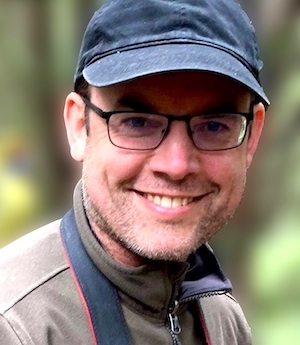
\includegraphics[width=0.2\textwidth,height=\textheight]{imagesForRmd/corellaOnShoulder2020croppedBlurredByAdobeOnline.jpg}

\hypertarget{attending-to-moving-objects}{%
\chapter{Attending to moving objects}\label{attending-to-moving-objects}}

\hypertarget{tracking-task-short-description-and-anecdotes}{%
\section{Tracking task short description and anecdotes}\label{tracking-task-short-description-and-anecdotes}}

On the road, drivers monitor the movements of others' vehicles. In conference halls, scientists monitor the position and posture of other researchers relative to the ones they are chatting to, in order to best time their approach. At the beach, parents keep watch as their children move in and out of the water. On the sports field, players often find themselves trying to keep track of multiple team-mates and opponents and their spatial relationships to the ball.

How do we do this and what does that tell us about how the mind works?

Until the late 1980s, almost no-one who studied attention used moving objects. Partly this was a technology issue, even though in 1979, the first popular home game console, the Atari, introduced Asteroids.

The task was to shoot and dodge the asteroids that are streaming in all directions. It pays to monitor more than one of the moving objects, to determine which way one should move, or shoot, to prevent a collision. Psychologists were slow to use the associated technology to study how people processed multiple moving objects. Finally, in 1988, \citet{pylyshynTrackingMultipleIndependent1988} used an Apple II+ computer to conduct an experiment that demonstrated that people could keep track of multiple moving objects. Pylyshyn \& Storm showed that people can keep track of multiple moving objects designated as targets in a crowd of identical distractors.

It was immediately apparent that the ability to track had a rather dramatic capacity limitation. That is, performance dropped quite rapidly as the number of targets was increased.

For the particular object trajectories and speeds used by some researchers
\citet{pylyshynTrackingMultipleIndependent1988}, performance dropped rapidly

This ability was also immediately observed to have a severe capacity limit.

Researchers quickly latched onto the word ``attentional'' to describe this ability,
in part because various

Along the way we will bust myths such as the common notion that people can track four or five objects,

Is object tracking just sustained attentional selection, when the objects happen to be moving? Well, a first question fundamentally is how do you keep your attention on the object? The literature on visual search is enormous but is almost exclusively about finding

Without continuous attentional selection, you not only lose your children

, and instead continued studying the processing of static, un-moving objects.

sticking with static, unmoving objects that

and other computer games with moving objects were introduced in 1979, psychologists were slow to use this technology to study how people process multiple moving objects.
Psychologists were slow to

Navigating a crowded street

And today, children frequently try to track rapidly moving objects in their own home - like many other things, tracking has come to screens.

For the generations of children since 1979, when Asteroids was invented,

You won't find much about this ability in chapters about visual attention. This is partly because for decades, the study of visual attention used only still, un-moving objects.

The study of visual attention took off in the 1970s with work by Eriksen, Treisman, . We learned an enormous amount about \emph{static} objects.

a huge topic, but

This will make the case for tracking being much more important than people realize. but you can't even perceive spatial relationships.

The manuscript would start with a few anecdotes illustrating why keeping track of objects is important both today (e.g., keeping track of one's children at the beach, keeping track of particular players on the sports field) and in evolutionary history (e.g., keeping track of the weakest members in a herd of prey). Then it would transition into some basic background about the visual system. Descriptions of the the draft sections are below. These section descriptions showcase that multiple, typically separate literatures would be integrated.

Cups and balls painting either here or in identity section, also with Saiki

\hypertarget{outline}{%
\section{Outline}\label{outline}}

\textbf{Intro}

\textbf{Bottlenecks}

\textbf{Which aspect(s) of tracking determine performance?}

\begin{enumerate}
\def\labelenumi{\arabic{enumi}.}
\tightlist
\item
  C=1 processes
\item
  Duration one can sustain attention
\item
  Spatial selection of multiple locations, even static ones
\item
  Spatial interference
\item
  Temporal interference
\item
  Speed limit of attention-following
\end{enumerate}

Each of these could hinder performance more with more targets. They contribute in an unknown mix to most trakcing tasks .
Thus we don't know which is responsible for various results. This has afflicted the quest to understand serialOrParallel,

\textbf{speed, and time.} The physical parameters that can limit tracking performance are space, speed, and time. Each plays a role in different circumstances, but the temporal limits are the most misunderstood, as I have discovered in reviewing journal manuscripts over the years, even though they may be the most fundamental. This section will explain spatial limits, speed limits, and temporal frequency limits on tracking (based in part on three papers from my lab), and how they illuminate other issues such as the relationship of tracking to basic motion and position perception.

Animated-horse-race-jockey.gif

\textbf{Serial processing, parallel processing, or both?} The way that our limited capacities are allocated over time to multiple objects, that is whether in parallel or in rapid series, has been a long debate. Recent evidence (including one of my papers) points to a serial component that seems to relate to natural oscillations in the brain, but much is yet to be determined.

\textbf{Identity}

including Vaziri-Pashkam et al.

\textbf{Mobile computation}

\textbf{Abilities}, Individual differences, dual-task interference, abilities

huangMeasuringInterrelationsMultiple2012. wilmerMultipleObjectTracking2016. Large differences have been found in spatial crowding, which probably explains a good chunk of the variance. Large individual differences in crowding have been established,

Nobody has yet

\textbf{Misconceptions and questions}

\textbf{Towards the real-world} and real-world tasks. A naive view of visual perception is that we are simultaneously aware of the identities of all the objects in a scene, so unless a player actually disappears or hides behind something or someone, we should know where everyone on the bacsketball court is at all times. Bringing together the factors described in previous sections, and bringing in new ones such as limits on feature binding, we will analyze some real-world tasks.

\hypertarget{twoBrains}{%
\chapter{Two brains or one?}\label{twoBrains}}

The fact that the brain is made up of two separate hemispheres has some striking consequences for object tracking , and more subtle ones for other tasks involving keeping objects in mind. This section will review the research regarding the remarkable hemifield independence of multiple object tracking (including two papers from my lab), as well as the specificity for spatial attention tasks - non-spatial measures of working memory show little independence, implicating a more unitary resource.

NOBODY has incorporated the hemifield division in their model!

Most people know that the brain has two hemispheres. Many know little else about the brain, but they understandably assume that the division of the brain into two halves has major consequences for how we learn. A major industry of pseudoscientific education consultants and brain training programs has sprung up around ideas such as ``left brain versus right brain'' training \citep{kroezeBrainGymPseudoscientific2016}. The truth is that while early sensory processing is very hemisphere-specific, more cognitive functions such as explicit learning benefit from remarkably tight integration of the two hemispheres. When we open our eyes, we have the experience of attending easily to objects in any part of the visual field. We experience no dislocation when the movement of our eyes, or of an object, cause it to shift from one hemifield, where it is processed by one hemisphere, to the other hemifield, where it is processed by the other hemisphere. Communication between the two hemispheres happens rapidly and continuously. There is little to no evidence that exercises designed to insure both hemispheres process stimuli have any benefit for learning.

For those extraordinarily rare individuals who have had some connections between their hemispheres cut (``split brain'' patients), the hemispheres act more independently. For tasks including searching for a target among many distractor objects, it is better to distribute the distractors across the two hemifields. Spreading the load in this way yields a large benefit for search, suggesting that both hemispheres can search independently and simultaneously. \citep{luckIndependentAttentionalScanning1994a}. But for normal individuals, no such advantage is seen, suggesting that the processes that evaluate each stimulus for whether it is the target are well integrated across the hemispheres \citep{luckIndependentHemisphericAttentional1989}. Yet for a few tasks, normal individuals act much more as if their hemispheres are working independently.

In visual short-term memory tasks, people perform a good deal better when the stimuli are spread across both the left and right hemifields rather than all presented to the left hemifield or to the right hemifield \citep{delvenneVisualShorttermMemory2012}. The reason, it is believed, is that there is some sort of resource that is specific to each hemifield. It is better, then, to spread one's load, rather than burdening one hemisphere more than the other. If the processes that limit memory performance were entirely specific to the hemispheres, then once people's limit for remembering objects presented to one hemifield were reached, one could add more objects to the other hemifield without any cost for the proportion of objects remembered. Instead, though, the hemifield advantage is only partial. There are a few tasks, however, for which the hemifield advantage seems to be complete, and multiple object tracking is one.

\citet{delvenneCapacityVisualShortterm2005}: ``a color and spatial location change detection task, in which the items were displayed either in the two visual fields or in the same hemifield. The data revealed that only memory capacity for spatial locations and not colors increased when the items were separated between the two visual fields. These findings support the view of VSTM as a chain of capacity limited operations where the spatial selection of stimuli, which dominates in both spatial location VSTM and MOT, occupies the first place and shows independence between the two fields.''

\citet{alvarezIndependentResourcesAttentional2005} were the first to show that distributing objects to two hemifields rather than one could, essentially, double performance, as if two brains were doing the task rather than one\ldots{}

\citet{hudsonHemifieldEffectsMultiple2012} multiple identity tracking , found a hemifield advantage: " Contrary to expectations, a bilateral advantage was still observed, though it was not as strong as when observers were not required to remember the identities of the targets. This finding is inconsistent with the only model of multiple identity tracking (Oksama \& Hyönä, 2008, Cognitive Psychology, 56, 237-283), so we present an alternative account."

\citet{strongHemifieldspecificControlSpatial2019}

RIGHT HEMIFIELD IS BETTER \citet{holcombeObjectTrackingAbsence2014} (Figure A2), Battelli

\hypertarget{quadrants}{%
\subsection{Quadrants}\label{quadrants}}

Carlson et al.~found evidence for quadrants. Has this been replicated? And \citet{strongHemifieldspecificControlSpatial2019} found a cost for crossing the vertical midline but not the horizontal midline. So now we know that the cross-hemisphere cost does not occur for quadrants.

\hypertarget{bottlenecks-and-capacity}{%
\chapter{Bottlenecks and capacity}\label{bottlenecks-and-capacity}}

How many arithmetic problems can you do simultaneously? Although your brain contains more than 80 billion neurons, if you are asked to multiply two two-digit numbers together, you will only be able to do one at a time \citep[\citet{zylberbergBrainRouterCortical2010a}]{oberauerAccessInformationWorking2002}. Of course, this is not a task that most of us do daily. Reading, however, is such a task. If I showed you twenty words on a page, how many could you read simultaneously? A large body of psychological research suggests that humans can read at most only a few words at a time, and some claim that we can only read one word at a time \citep{whiteEvidenceSerialProcessing2018, reichleEncodingMultipleWords2009}.

Some parts of the mind can process many things at once. In vision, early processing stages are massively parallel. Each bit of the retinal image has its own photoreceptors devoted just to it. In the primary visual cortex, individual neurons respond to larger regions, but collectively still process many regions at once, in parallel.

A common example of a visual ability that appears to have a high simultaneous processing capacity is a certain kind of visual search. In some circumstances, we can quickly locate targets hidden in a large number of distractors. For example, try searching for the blue objects in the below display.

\includegraphics{tracking-review_files/figure-latex/unnamed-chunk-3-1.pdf}

Locating the three blue objects should be very easy. One reason is that our visual systems process each of the shapes simultaneously, and makes the locations of the blue objects available when you choose to attend to blue. Some brain areas, however, do not have neurons that can recognize objects dedicated to each bit of the visual field. Instead, their simultaneous processing capacity is limited. The processes required to recognize words are an example.

For limited capacity processes, something is needed to pick out, from a crowded scene, just one or a few objects for these areas to recognize. We call this something \emph{selective attention}. Different visual abilities seem to have different capacities, and it is not at all clear that a common selective attention process is responsible for gating all of their inputs.

\citet{duncanSelectiveAttentionOrganization1984} was interested in how many objects we can process at a time. He found that accuracy for making a simple visual judgment about an object was much worse when one needed to simultaneously make a judgment about another. For example, participants were asked to judge whether a briefly-presented rectangle was small or large and also judge whether a simultaneously presented line was dotted or dashed. Performance was worse in the two-object condition even in comparison to a single-object condition where two judgments also needed to be made. The participants had to make either two judgments about a single object or one judgment about one object and the second judgment about a different object. To Duncan, his finding that performance was substantially worse in the two-object condition indicated the existence of a bottleneck at a stage that processes objects. He wrote that

\begin{quote}
Findings support a view in which parallel, preattentive processes serve to segment the field into separate objects, followed by a process of focal attention that deals with only one object at a time.
\end{quote}

This conclusion was a bit of an over-reach. Performance was better than one would expect if only one object were processed, unlike what has been found for word processing. Duncan could explain that by saying that the presentation time was adequate for focal attention to, on \emph{some} trials, process more than one object. Alternatively, however, it may be that the relevant processes \emph{can} handle two objects at a time, but just does so more poorly than for one object. Work that credibly claims that a visual ability is truly limited to one object at a time is hard to find; the reading of words may be an exception.

\hypertarget{the-tracking-bottleneck}{%
\section{The tracking bottleneck}\label{the-tracking-bottleneck}}

\hypertarget{there-is-no-hard-limit-on-the-number-of-objects-that-people-can-track}{%
\subsection{There is no hard limit on the number of objects that people can track}\label{there-is-no-hard-limit-on-the-number-of-objects-that-people-can-track}}

Like reporting on the features of objects, the processing needed to covertly track objects also has very limited capacity. Participants asked to track several objects perform much worse than if they are asked to track only a few objects.

The tracking bottleneck implied by such results is frequently portrayed in the literature as being a hard limit, or close to it. \citet{doranRoleVisualAttention2010}, for example, claim that ``the main finding'' from the object tracking literature ``is that observers can accurately track approximately four objects and that once this limit is exceeded, accuracy declines precipitously.'' , \citet{fougnieDistinctCapacityLimits2006} write that ``People's ability to attentively track a number of randomly moving objects among like distractors is limited to four or five items'', \citet{piazzaNeurocognitiveStartupTools2011} state that ``One of the defining properties of this system is that it is limited in capacity to three to four individuals at a time'' , \citet{alvarezHowManyObjects2007} that "``researchers have consistently found that approximately 4 objects can be tracked'', \citet{chesneyEvidenceSharedMechanism2011} write that ``people typically can track four or five items'' , and \citet{vanderburgChangesNotDifferences2019} write that ``participants can track about four objects simultaneously'' . In each of these cases, I have checked the evidence provided, or the papers cited, as well as the papers those papers cite. Each paper either provides no relevant evidence, or finds instead only a gradual decrease in performance as number of targets is increased with no discontinuity, nor even a conspicuous inflection point. For example, \citet{oksamaMultipleObjectTracking2004} designated between two and six objects as targets, among twelve identical objects in total. After the objects moved around randomly for five seconds, one object was flashed repeatedly and participants hit a key to indicate whether they thought it was one of the targets. The proportion of trials in which participants were wrong increased steadily with target size, from 3\% incorrect with two targets, to 16\% incorrect with six targets. Note that even with six targets, participants were performing substantially better than would be expected if they could only track one or two and had to guess on the others.

Some of the spurious claims of a limit for tracking of about four objects seems to stem from wishful thinking by researchers that the capacity limit on various tasks might co-incide. The literature on numerosity perception had long found a discontinuity in performance for estimating the number of collections of more than about four objects \citep{jevonsPowerNumericalDiscrimination1871, revkinDoesSubitizingReflect2008}. In the ``subitizing range'' of four or fewer objects, performance is approximately as good for rapidly counting four objects as it is for two or one. This appears to have motivated researchers to suggest, sometimes with little evidence, that other tasks show the same phenomenon of a very high performance below a particular number of objects, with a steep decline after. For example, in the Introduction of \citet{bettencourtSharedFilteringProcesses2011}, the authors write ``both processes {[}visual short-term memory and MOT{]} showing an equivalent four-object limit''.

\hypertarget{there-is-no-real-limit-on-the-effective-number-of-objects-that-people-can-track}{%
\subsection{\texorpdfstring{There is no real limit on the \emph{effective} number of objects that people can track}{There is no real limit on the effective number of objects that people can track}}\label{there-is-no-real-limit-on-the-effective-number-of-objects-that-people-can-track}}

A very widespread idea in the

Many cognitive psychology researchers, even those that have never read a paper

ill-formed question?

This has been the dominant framing since the beginning of MOT research, when Pylyshyn suggested that tracking was limited by the number of discrete pointers or FINSTs that people have. But the underlying reason for variation in MOT performance may not be due to variation in number of FINSTs or some other such capacity, but rather due to variation in peoples' tracking speed limit, spatial interference, or temporal interference. This does not seem to have been properly investigated.

This question is a mistake.

Working off the dominant framing, that each person does have a specific number of targets they can track which determines percent correct for each level of number of targets, some MOT researchers report what \citet{schollWhatVisualObject2001} called the ``effective number of items tracked''. The associated formula, refined by \citet{hullemanMathematicsMultipleObject2005a} allows researchers to calculate the effective number of items tracked based on accuracy in an individual condition, given the number of targets and distractors in that condition. This does provide a useful summary of the data, but researchers should take more care to avoid taking it literally.

\citet{meyerhoffIndividualDifferencesVisual2020} tested fifty participants and for each one calculated the effective number of items tracked, for a display with four targets and four distractors, the modal effective number of items tracked was around two, but a substantial proportion of participants's came in at three targets or one target, and a few scored close to zero effective items tracked.

Unfortunately, in the data of \citet{meyerhoffIndividualDifferencesVisual2020}, like that of many others, there is no way to know how much of the variation between individuals is due to motivation rather than ability. Measuring motivation is not easy, but researchers should at least include what are sometimes called attention checks or catch trials to allow exclusion of participants who show clear evidence of not reading the instructions carefully or frequently not paying attention.

The statements in the literature such as ``participants can track four moving objects'' also mislead readers in another way. The finding that participants can track at least four objects with reasonable accuracy is restricted to particular object speeds \citep{alvarezHowManyObjects2007, holcombeExhaustingAttentionalTracking2012} and spacings \citep{franconeriEvidenceSpeedLimit2008, holcombeObjectTrackingAbsence2014}.

The particular number of objects that can be tracked with reasonable accuracy is thus highly dependent on conditions. Still, it is clear that this number is small relative to the number of objects that are simultaneously processed by early stages of the visual system. So, what aspect exactly of tracking imposes this limitation?

\hypertarget{objects}{%
\chapter{Objects}\label{objects}}

Keeping track of something that is moving implies that our mind is continually, or at least frequently, updating a representation of its position. Most researchers seem to conceive of this as keeping spatial attention on an object, a sort of spotlight or hill of neural activation that glides across retinotopic cortex. There is evidence for this from neuroimaging. In this article, for simplicity we will refer to the spatial index that changes along with a moving object as a spotlight of attention. This spotlight account is consistent with evidence that probes are more easily detected on targets than elsewhere \citep{pylyshynPuzzlingFindingsMultiple2006, searsMultipleObjectTracking2000}. Keep in mind, however, that we do not mean that a hill of activation in spatiotopic or retinotopic cortex exhausts all the processes involved in tracking - there are certainly more.

How does the brain manage to shift attention along with an object? As an object moves, what causes the spotlight of attention to move along with it, rather than staying in place? Several decades of work on attention have robustly documented the existence of spatial selection and feature selection. That is, when people are instructed to think about a particular location in the visual field, this results very rapidly in facilitation of perceptual performance for that location, and neural activation in the associated parts of retinotopic cortices. There does not seem to be any ``search'' needed, instead spatial location seems to provide a direct conduit for attentional activation. Similarly, for certain features such as motion and color, an instruction to attend to a particular direction, or a particular color, triggers rapid activation across the visual field at all the locations of that particular color or motion \citep{saenzGlobalFeaturebasedAttention2003, whiteFeaturebasedAttentionInvoluntarily2011}.

What role do spatial and feature attention play in object tracking? If a moving target differs from distractors in certain ways, then feature attention can be relied on to keep attention on the target. For example, if the targets are the only yellow objects in the scene, and all the distractors are blue or green, then one might be able to think ``yellow'' and that would be enough to keep attention on target. However, when the targets are identical to the distractors, some other process is needed. One possibility is ``object-based attention''. Now, no one seems to think that object \emph{selection} is a thing. That is, one cannot think ``chair'' and expect all the locations of chairs in the scene to rapidly be attended. No, selection of chairs seems to require a search first, based on locations and simpler features.

\hypertarget{attentional-spread}{%
\section{Attentional spread}\label{attentional-spread}}

However, what might be the case is that once one \emph{is} attending to an object, some process causes one to attend to the entire object, rather than just one or a few individual locations on it. This does seem to happen, and shows up in experiments where one end of a (static) object is cued, which results in facilitation not only for probes at that end of the object, but also at its other end \citep{eglyShiftingVisualAttention1994a}. This pattern is not always observed, so this is not fully understood \citep{davisReversalObjectBased2005, shomsteinObjectbasedAttentionStrength2008, shomsteinObjectbasedAttentionSensory2002, louIndividualDifferencesTemporal2020}, but perhaps the best explanation is that attention often does tend to spread to an entire object.

A ``spread'' of attention, or gradual growth of the area of attentional activation to encompass an entire object, is not the only conceivable process that might yield object-based attention benefits, but such spreading has been observed neurophysiologically in certain tasks \citep[e.g.,][]{wannigAutomaticSpreadAttentional2011}. Such a spreading process might explain the ability to keep attention on multiple moving objects.

When an object moves, if it moves smoothly, then its leading edge will occupy new territory while its trailing edge continues to occupy an old location. If spreading of attention up to object boundaries is continually occurring, then attention should spread to the new locations near the trailing edge. In such a fashion, attention could, by continually expanding to the new location of a leading edge and contracting with a trailing edge, stay on a moving object. Some problems with this account, discussed in SECTION X , suggest that spreading of attention is not sufficient to explain tracking, but it may play a role.

Not all aspects of our attention automatically spread throughout an object. Imagine viewing a distant tree on the horizon, silhouetted by a setting sun. One can choose to attend to the top of the tree, a part of its trunk, or perhaps an individual branch. One seems to be able to focus attention on an arbitrary spatial region, even if it is only an undifferentiated portion of a larger object. But experiments find that the processes that mediate tracking do not have the capability to do that. This was demonstrated in striking fashion in experiments reported by \citep{schollWhatVisualObject2001}.

\citet{schollWhatVisualObject2001} asked participants to track, among other things, ends of lines. That is, they presented participants with four lines and designated one end of each as a target. The participants' task was to keep track of those four ends and at the end of the trial indicate which line ends were targets by clicking on them with the mouse. During a trial, each line grew, shrank, and rotated as each of its ends wandered about the screen randomly.

\begin{figure}
\centering
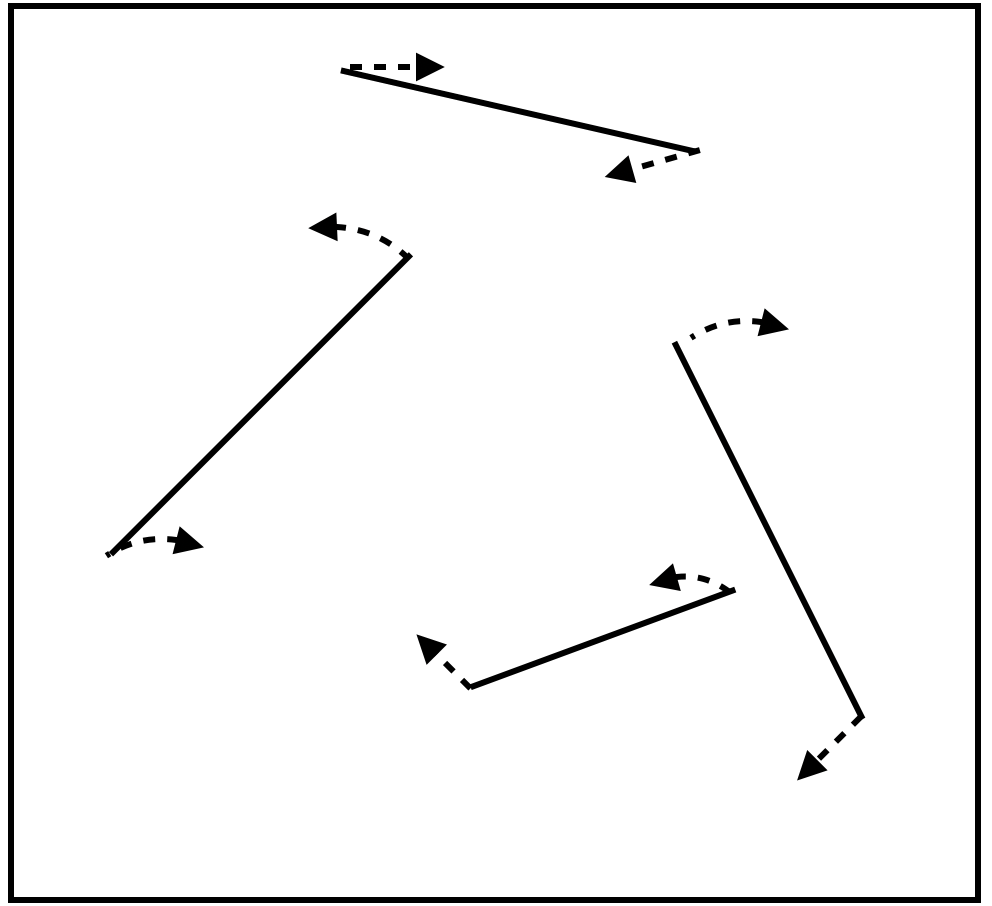
\includegraphics[width=0.4\textwidth,height=\textheight]{imagesForRmd/linesSchollPylyshynFeldman_madeByHolcombe.png}
\caption{A schematic of the display used by Scholl et al. (2001)}
\end{figure}

Performance on this task was abysmal relative to a control condition in which the two ends of the line were not connected. When viewing an example trial, many people can quickly feel how difficult the task is.

INSERT MOVIE

Follow-up work by \citet{howeCanAttentionBe2012} showed that the changing length of the lines is not the reason for the difficulty, which supports the interpretation that one cannot confine one's tracking processes to one bit of an undifferentiated object.

\hypertarget{are-object-creation-processes-distinct-from-tracking-processes}{%
\section{Are object creation processes distinct from tracking processes?}\label{are-object-creation-processes-distinct-from-tracking-processes}}

In the literature, commonly the word ``attention'' is used to refer both to the processing that determines how many things one can track and for the processes that determine what kinds of things can be tracked. However, a popular notion is that these processes are quite distinct, with processes prior to tracking determining what counts as an ``object'' (a thing one can track), with subsequent stage(s) limiting how many such objects one can track. This is often how the processing for other tasks such as visual search has been conceptualized, with some empirical support (\citet{wolfePreattentiveObjectFiles1997}, \citet{nakayamaVisualSurfaceRepresentation1995}), and appears to be the position assumed by \citep{schollObjectsAttentionState2001} in his review of objects and tracking.

USE diagrammeR OR POWERPOINT TO MAKE A BOX DIAGRAM OF THIS, WITH OBJECT FORMATION PRIOR TO TRACKING

It would be convenient if this view were correct, because studying a system comprising distinct stages is more straightforward than understanding a more interactive system \citet{simonSciencesArtificialReissue1969} pp.~99-103?, but I do not know of any good tests of this conjecture. One complication for exploring the issue is that one is \emph{not} always unable to track an undifferentiated part of an object. In particular, the limitation is somewhat restricted to when one is attempting to track \emph{multiple} objects.

Watch the above movie again, this time concerning yourself with keeping track of the end of only \emph{one} object. You are likely to succeed. Indeed, \citet{schollObjectsAttentionState2001} found that if participants are asked to track four line ends, their performance is very poor (athough still somewhat better than chance). Specifically, their performance was approximately that predicted if they could track one line end, but not more. This suggests there are tracking-relevant abilities that we have that can be brought to bear on one thing, but not multiple things. Perhaps covert multiple object tracking (MOT) is qualitatively different, then, from covertly tracking a single object.

Another possibility is that the same underlying resource is involved in both the ability to track one undifferentiated part of one object and the ability to track multiple objects. On this account, rather than a different \emph{kind} of resource allowing tracking a part of an object when there is only one to track, instead there are simply \emph{more} resources needed to track an undifferentiated part of an object. We will return to this possibility in \ref{twoBrains}.

\hypertarget{objects-and-object-hood}{%
\section{Objects and object-hood}\label{objects-and-object-hood}}

The study of how the visual system segments a scene into objects or groups has a long history. The Gestalt psychologists sought to discover what cues cause separated visual elements to appear to be grouped together. Developmental psychologists took

The near-impossibility of tracking the ends of multiple lines invites the question of what else

It could be that what determines what objects are is a separate set of processes than those that actually do the tracking. This is what is advocated by Scholl.

What is a moving object? People, animals, cars, leaves, and balls are all objects that change position smoothly and that we can keep track of in a crowd. But how do our brains

The water of a river, a creeping shadow, a slinking Slinky, an oozing

TRANSITION TO NEXT SECTION:

\hypertarget{finish}{%
\section{FINISH}\label{finish}}

This proposition, that there are actually two resources that can assist tracking, one with much more limited capacity (perhaps for just one object) and the other with fewer capabilities but higher capacity, is an intriguing one but not

A word of caution, however - because tracking performance decreases

Those abilties of ours that have a capacity of just one remain somewhat obscure. There is an extensive literature on two-object costs. words Alex White However,
However, as we will see in velocityAndExtrapolation, there is evidence that some aspects of motion processing

Some mental processes seem to have a capacity of just one. That is, there are abilities we have that can be

Mention the bendy-pencil illusion \url{https://jov.arvojournals.org/article.aspx?articleid=2193187} and Gershman's hierarchical paper
From the bendy-pencil illusion paper: ``One of the basic discoveries of Gestalt psychology is that the perceived trajectory of a moving object is not always determined by its relative motion with respect to the retina or the ground but may instead be based on its motion relative to other moving objects. The perceived motion of a rolling wheel provides an excellent example (see Duncker, 1929; Johansson, 1950; Rubin, 1927, for more examples). The trajectory of a single point on the wheel has the form of a cycloid, but its perceived trajectory is a simple rotary motion about the center of the wheel. Indeed, it is not possible to perceive the cycloidal trajectory, even if one tries, unless the point is presented in isolation.''

\hypertarget{which-aspects-of-tracking-determine-performance}{%
\chapter{Which aspect(s) of tracking determine performance?}\label{which-aspects-of-tracking-determine-performance}}

Why do people perform more poorly with more targets? The processes involved must be, by definition, capacity-limited in that they do worse with more targets. But what aspect of the tracking task does lack of capacity cause them to suffer from more?

Below is a list of candidate reasons for the factors that impair performance more when there are more targets:
In a typical MOT task, any of the below are candidates for being one of the reasons, or the main reason, that performance declines with number of targets:

\begin{enumerate}
\def\labelenumi{\arabic{enumi}.}
\tightlist
\item
  General cognition
\item
  Duration that one can sustain attention
\item
  Spatial selection of multiple locations, even static ones
\item
  Spatial interference
\item
  Temporal interference
\item
  Speed limit of attention-following
\end{enumerate}

This section will explain what is meant by each of these factors. The most important of them will be discussed in more detail in subsequent sections.

\hypertarget{c1-processes}{%
\section{C=1 processes}\label{c1-processes}}

In introducing the concept of a bottleneck or capacity limit in the previous section, I used the example of math problems. Using our capacity for reasoning and symbol manipulation, we can perform a wide array of arbitrary tasks. We therefore should not be surprised by our ability to track a \emph{single} target. We know that we have a visual system that makes the position and direction of motion of objects on our retina available to cognition, and that using our ability to think about where an object is going and deliberately move our attention to a future anticipated location, we might muddle through tracking a single object. For purposes of illustration, let us call the processes involved ``C=1 processes'' to reflect the possibility that some cognitive processes involved have a capacity of only one object.

Oberauer

What makes MOT interesting to many is that we can track more than one target. This implicates the involvement of another, higher-capacity sort of processing. The contribution to MOT of two kinds of processing, with different capacity limits, complicates the interpretation of MOT results. Even when participants are asked to track several targets, one can expect that C=1 processes are contributing to overall performance, even if they are only involved in the processing of one of the targets.

Thus, when researchers contrast tracking performance with different numbers of targets, one reason for the decline in performance may be that C=1 processes are, in each condition, processing only a single target, so performance declines in inverse proportion to the number of targets.

\hypertarget{duration-that-one-can-sustain-attention}{%
\section{Duration that one can sustain attention}\label{duration-that-one-can-sustain-attention}}

Tracking may be, in part, a test of how long one can sustain attention. There also is some possibility that additional demands on attention (more targets) reducing the average amount of time one can sustain attention without a lapse. The results of \citet{wolfeMultipleObjectJuggling2007}, suggest that this need not be the case. In their Experiment 3, participants were required to track four targets for a period of ten minutes. Every 9 seconds or so, one object was highlighted and participants had to indicate whether it was one of the targets. In a no-feedback condition, participants were not told whether their individual responses were correct. In that situation, performance was substantially worse in the last few minutes of the trial than in the first few minutes (78\% correct vs.~65\% correct). However, in the feedback condition wherein participants were told immediately after each judgment whether they were correct, performance did not appear to decline over time. These results suggest that if participants are adequately motivated by feedback, they have considerable ability to track for several minutes with no appreciable loss. The comparison between the feedback and no-feedback conditions is not perfect as the feedback does provide a cue that can increase performance (when participants get the probe wrong, they can increase subsequent performance somewhat by switching to another target), but this confound does not seem to be able to explain the lack of almost any performance loss in the feedback condition.

The circumstances used by \citet{wolfeMultipleObjectJuggling2007} were quite different from a prototypical MOT task, not least because of the extended durations of the trials. Most researchers use trial durations of less than 10 seconds, and it is not clear whether the \citet{wolfeMultipleObjectJuggling2007} results would generalize. It seems likely that participants can attend for several seconds without losing much motivation, but \citet{oksamaMultipleObjectTracking2004} found a substantial decrease in performance for trials of 13 s compared to trials of 5 s. With four targets, for example, performance fell from 91\% correct to 74\% correct, and this decrease was somewhat greater for larger numbers of targets than for fewer targets. Byrne \& Holcombe (unpublished data) did not find any significant decrease over a comparable interval, and the explanation for these discrepancies is uncertain, although it may again be related to participants' motivation.

The reason for the reduction in performance with greater time observed by \citet{oksamaMultipleObjectTracking2004} may easily be due to another factor rather than an increase in lapses of attention. In the MOT tasks used by all of these researchers, with longer trials there is likely to be more instances of potential spatial interference, temporal interference, and running afoul of any attentional speed limit. Thus, if any of those factors matter, they could explain the decrease in performance with time. However, the \citet{wolfeMultipleObjectJuggling2007} does seem to provide a kind of existence proof that lapses of attention need not be the limiting factor. Granting that that may be the case, an additional question is why, if other factors are in operation, there was \emph{no} evidence of a performance decrease over time in \citet{wolfeMultipleObjectJuggling2007}? Well, \citet{wolfeMultipleObjectJuggling2007} averaged performance over approximately the first third of the ten-minute interval and compared it to the last third. In the feedback condition, it is possible that all the worst possible events (such as close approaches, causing greater spatial interference) had already occurred by the end of the first third, so whatever level of performance participants were left with at that point already reflected their capacity to track through the most difficult events, which they were then able to continue to do until the end of the trial. Over a shorter time range such as that used by \citet{oksamaMultipleObjectTracking2004}, this may not have been the case.

\hypertarget{spatial-selection-of-multiple-locations}{%
\section{Spatial selection of multiple locations}\label{spatial-selection-of-multiple-locations}}

At the beginning of an MOT task, featural attention is typically used to select the target objects, as they are typically highlighted with a different color or by flicker. Both \citet{drewNeuralMeasuresIndividual2008} and \citet{franconeriHowManyLocations2007} found evidence that this was not as demanding as the motion phase of the tracking task. However, the selection phase may still be demanding enough to result in incorrect responses on many trials, and thus affect overall performance, and do so to a greater extent when there are more targets.
In the experiments by \citet{franconeriHowManyLocations2007}, participants two concentric circular arrays of dots centered on fixation. Between one and eight of these dots were briefly highlighted, and then each dot was replaced by either a small horizontal or a small vertical bar. The participants' task was to search for a vertical bar, but to confine their search to only the previously-cued locations. They pressed one key if a vertical bar was present among the cued locations, and another key if none of those locations contained a vertical bar.

In a relatively easy condition (a sparse condition with only 12 locations), average performance dropped from 98\% for two cued locations to 91\% for six locations. Such a small decrease suggests that if this result were to generalize to typical MOT displays, the selection phase would contribute only a small portion of the performance decrease with greater set sizes. MOT displays typically do only have 12 or fewer objects. However, they frequently are much closer to each other than the spacing that \citet{franconeriHowManyLocations2007} used in their sparse condition. In the denser conditions tested by \citet{franconeriHowManyLocations2007}, performance again started at a very high level for two cued locations, but dropped much more, to 74\% correct or less for six cued locations.

The initial selection demands in a typical MOT task are likely less taxing than in these experiments, because participants need only maintain their attention on the objects, not search through them. However, it is not clear how much less demanding maintained attention is, so we still do not know how much of the target-number effect in typical MOT displays is due to failures at the very beginning of a trial. The density effect observed by \citet{franconeriHowManyLocations2007} suggests a role for spatial interference in typical MOT experiment, which is the factor we turn to next.

\hypertarget{spatial-interference}{%
\section{Spatial interference}\label{spatial-interference}}

\hypertarget{temporal-interference}{%
\section{Temporal interference}\label{temporal-interference}}

Temporal interference is analogous to spatial interference, just in time rather than in space. Spatial interference refers to a processing impairment when one object comes closer than a certain spatial distance to a second object, at one time. In contrast, temporal interference refers to when an object comes closer than a certain temporal distance of another, at one point in space.

The objects in typical MOT displays often travel over locations formerly occupied by another moving object. That is, after one object passes over a location, another will pass over the same location, some amount of time later. If temporal interference is a factor in object tracking, then if the amount of time that separates the two objects occupying a location is short enough, tracking will be impaired.

If objects are moving fast enough, they are perceived to blur together, because some parts of the visual system integrate over several dozen milliseconds \citep[e.g.,][]{hogbenPerceptualIntegrationPerceptual1974}. A more interesting question is whether temporal interference occurs on a longer timescale, more relevant to the speeds and spacings typically used in MOT tasks.

\hypertarget{speed-limit-of-attention-following}{%
\section{Speed limit of attention-following}\label{speed-limit-of-attention-following}}

\hypertarget{moving-forward}{%
\section{Moving forward}\label{moving-forward}}

Each of these could hinder performance more with more targets. They contribute in an unknown mix to most trakcing tasks .
Thus we don't know which is responsible for various results. For example,

\hypertarget{spatial-interference-1}{%
\chapter{Spatial interference}\label{spatial-interference-1}}

Long before \citet{franconeriHowManyLocations2007} conducted experiments on the selection of multiple locations with different densities, researchers had recognized the existence of spatial interference in dense displays \citep{wolfordPerturbationModelLetter1975, korteUberGestaltauffassungIm1923, strasburgerDancingLettersTicks2014}.

\hypertarget{htmlwidget-4d8d17bd518ed857095e}{}

If you gaze at the central dot in the above display, you likely will be able to perceive the middle letter to the left fairly easily (it is a `J'). However, if you again keep your eyes fixed on the central dot, but this time try to perceive the central letter to the right, it should be much more difficult. This is called ``crowding''.

Crowding refers to the spatial impairment of visual processing caused by stimuli that are near a target stimulus. It has been studied extensively in experiments that typically ask a participant to identify a single, motionless, briefly-presented stimulus such as a letter. Those studies have shown that crowding can be avoided if the flanking stimuli are presented sufficiently far away from a target. That distance varies depending on the display spatial arrangement and on the person, but on average extends to about half the eccentricity of the target, with the interference diminishing rapidly as separation increases beyond that \citep{boumaInteractionEffectsParafoveal1970a, gurnseyCrowdingSizeEccentricity2011}. For example, in the display above, the letters on the same side as the `J' are separated from it by more than half the 'J's distance from the fixation point, so they have little to no effect on its identification.

The psychophysical literature on crowding uses almost exclusively
In However, crowding also can prevent attentional selection from individuating a target. \citep{intriligatorSpatialResolutionVisual2001}

The overwhelming majority of MOT papers use trajectories for which targets frequently come within the crowding distance of another target or distractor. As a result, crowding likely contributes to tracking performance. In addition, crowding appears to be subject to substantial individual differences \citep{petrovAsymmetriesIdiosyncraticHot2011}, including larger crowding zones in a subpopulation of persons with dyslexia \citet{jooOptimizingTextIndividual2018}, so it likely also explains some of the variation in tracking performance between people.

\citet{franconeriTrackingMultipleObjects2010a} claimed that spatial interference is the \emph{only} reason why performance is worse when more targets are to be tracked, denying any role for speed, time, or any non-spatial form of processing capacity. Moreover, \citet{franconeriTrackingMultipleObjects2010a} implied that this interference extends over a much greater distance than the crowding range documented in the psychophysics literature. HOWEVER, \citet{franconeriTrackingMultipleObjects2010a} did not succeed in isolating the distance between objects, and careful parametric variation of separation has found evidence for tracking interference only within the crowding range \citep{holcombeObjectTrackingAbsence2014, holcombeExhaustingAttentionalTracking2012}.

However, what remains under-studied is whether, or by how much, the crowding range increases with the number of objects that should be monitored. A psychophysical study of crowding with briefly-presented stimuli found good evidence that attending to additional targets within the crowding range of a first target did result in a stronger crowding effect \citep{mareschalAttentionalModulationCrowding2010}. However, they did not measure how much further crowding extends.

\citet{holcombeObjectTrackingAbsence2014} compared tracking performance for one targets and two at various separations between the target trajectories.

and didn't find evidence that crowding extended further with two targets than with one,

\citet{maki-marttunenDistinctNeuralMechanisms2019}:``In both cohorts, increased load and close encounters (i.e., close spatial proximity) led to reduced accuracy in an additive manner. Load was associated with pupil dilations, whereas close encounters were not. Activity in dorsal attentional areas and frequency of saccades were proportionally larger both with higher levels of load and close encounters. Close encounters recruited additionally ventral attentional areas that may reflect orienting mechanisms. The activity in two brainstem nuclei, ventral tegmental area/substantia nigra and locus coeruleus, showed clearly dissociated patterns. Our results constitute convergent evidence indicating that different mechanisms underlie processing challenges due to load and object spacing.''

\hypertarget{moving-forward-1}{%
\section{Moving forward}\label{moving-forward-1}}

Each of these could hinder performance more with more targets. They contribute in an unknown mix to most trakcing tasks .
Thus we don't know which is responsible for various results. For example,

\hypertarget{serial-processing-parallel-processing-or-both}{%
\chapter{Serial processing, parallel processing, or both?}\label{serial-processing-parallel-processing-or-both}}

Brains are massively parallel, which has led many to be skeptical that anything has to be done in series, one-by-one. The evidence reviewed above strongly indicates that resources are limited and have to be shifted from object to object for certain tasks, this is compatible with multiple objects being processed at once, in small sets. But evidence emerged some time ago that certain task elements can only be processed by the brain one at a time.

One can certainly walk and chew gum at the same time, and even simultaneously use one hand to rub one's belly and the other to tap one's head, although it may take a bit of practice for some of us. However, when it comes to making a keypress based on the identity of a visual stimulus with one hand and based on the identity of a sound with the other hand, the evidence suggests that one particular component of these two tasks simply cannot be done simultaneously \citet{pashlerDualtaskInterferenceSimple1994}. Specifically, the pattern of response times indicates that while a choice is being made in response to the visual stimulus, choice processing for the auditory stimulus cannot commence.

From the beginning of the literature on multiple object tracking, researchers have debated whether any constituent process is limited to one-by-one processing\ldots{}

Unitary focus of attention in VWM, according to Oberauer, which would help explain the inter-individual correlation with WM performance.

Hybrid serial-parallel Bello model.
It's possible that tracking greater than the subitizing range requires significant VWM. Franconeri showed you often are wrong about how many targets.

\hypertarget{beyondLocation}{%
\chapter{Beyond location}\label{beyondLocation}}

How well are other features besides position tracked?

Blaser Pylyshyn Holcombe

\hypertarget{velocity-and-extrapolation-not-just-position}{%
\section{Velocity and extrapolation, not just position}\label{velocity-and-extrapolation-not-just-position}}

The role of motion signals . Seiffert

\citet{fencsikRoleLocationMotion2007} \citet{howeMotionInformationSometimes2012} both found evidence that motion is used for one or two targets but not more

Lack of extrapolation:

\citet{fencsikRoleLocationMotion2007} found it for one and two targets but not more

\citet{howardPositionRepresentationsLag2011} included a review of the literature on keeping up with current position. Eye movements lag - \citet{lukavskyGazePositionLagging2016}

Ryo Nakayama attention inertia theory

What about updating of features? Well, updating of surface features seems to generally be crap, e.g.~identity tracking is crap, Pailian

Integration:
Relation to oscillations

\hypertarget{speed-and-time}{%
\chapter{Speed and time}\label{speed-and-time}}

In our list of

How fast can people track? This is an important question, not only for predicting what people will be able to do in the real world, but also because investigations of the limits on tracking have led to insights into the relation of tracking processes to other aspects of attention and of motion perception.

\hypertarget{speed}{%
\section{Speed}\label{speed}}

Extrapolation theory predicts

\begin{itemize}
\tightlist
\item
  attention will be right on the target.
\item
  Linear effect of velocity
\end{itemize}

\hypertarget{time}{%
\section{Time}\label{time}}

What makes a tracking task hard for a person, or even impossible?

Let's return to the classic shell game. In a shell game, an item is placed beneath one of three identical shells, making that shell the target. The viewer tries to keep track of which shell has the item underneath it.

\begin{figure}
\centering
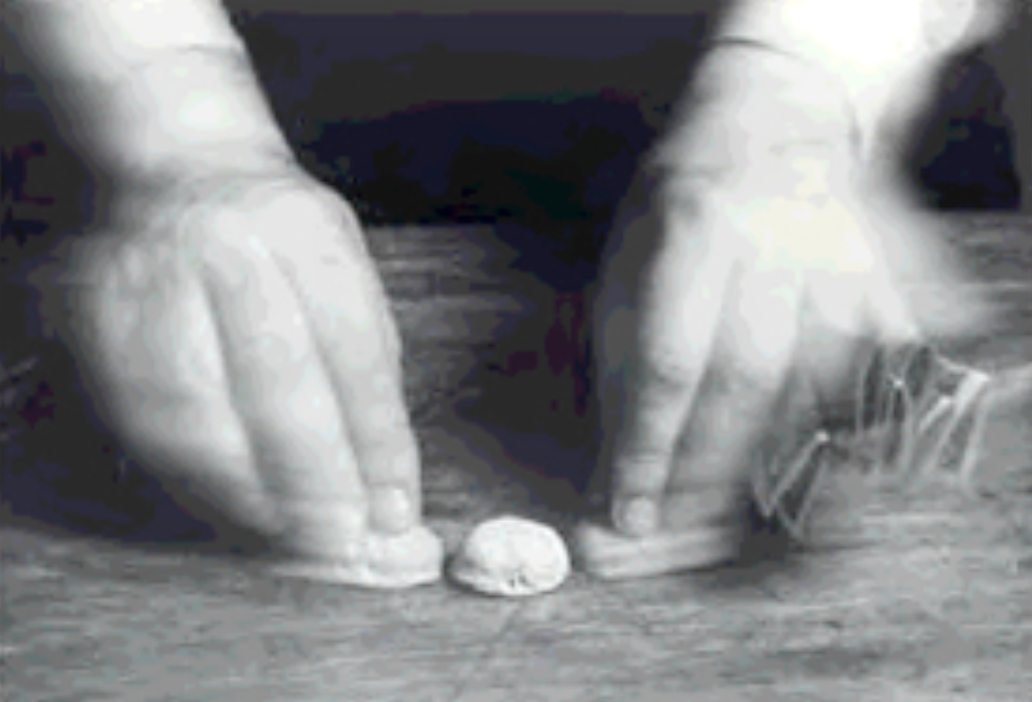
\includegraphics[width=0.5\textwidth,height=\textheight]{imagesForRmd/shellGame.png}
\caption{The location of two identical shells are exchanged in a shell game}
\end{figure}

A crucial aspect of the game is that the shells exchange locations with distractors. Thus, remembering the original location of the item is not sufficient. Neither is it sufficient to extrapolate a new position for the target based on the item's first direction of motion. Remembering its relative location in the array (e.g., the ``middle one'') is also not enough. One really must update one's representation of the target's position, rather than relying on any of the above.

The simple reduced laboratory version of the shell game is illustrated by the following schematic.

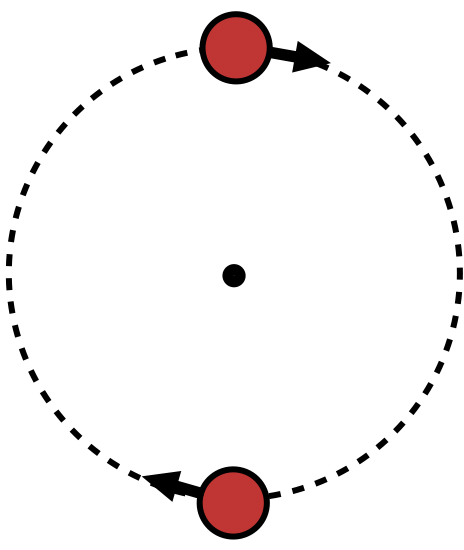
\includegraphics[width=0.1\textwidth,height=\textheight]{imagesForRmd/twoDiscsRevolving.png}

The updating of target position could fail for any of a few different reasons. A target might move too quickly for attention to move with it. That is, there may be a speed limit beyond which object position is not appropriately updated. Under serial switching accounts, this speed limit might occur if between successive samples, the object moved further than a critical distance between samples. Under parallel theories, the tracking process may simply have a speed limit. If the speed of the tracking process is resource-intensive, this speed limit may be slower when more targets are to be tracked.

\hypertarget{temporal-limits}{%
\section{Temporal limits}\label{temporal-limits}}

Another possibility is that tracking has a temporal limit, much like it has a spatial limit. Recall that in section X we described evidence that if a target comes too close to another object, the two objects can get confused. They won't always be confused, because predictable trajectories and target velocity can be used to recover a target even after it completely overlaps with another (\citet{howeMotionInformationSometimes2012}; Vul under review at JoV).

So, spatial confusions contribute to tracking. Might this also be the case for temporal confusions? There is already reason to think that
SHOW TICS-TYPE DEMO
Clearly there are some visual processes that are disrupted if other stimuli soon occupy the former location of an object. Perception of the object's color itself is still ok (Nishida ; \citet{cavanaghMobileComputationSpatiotemporal2008}). But

Spatiotemporal window account.
wapping errors presumably come about be- cause a target and a distractor approach within the width of the attentional window.

One might lose the target because it simply moves too fast to track. Or one could lose it because it came so close to a distractor in peripheral vision that they could not be spatially discriminated. These possibilities of a speed limit and of spatial interference have been well-appreciated by researchers. A third possibility has been less appreciated: a temporal limit.

While temporal limits are less familiar, they are the chief limitation on the perception of motion. The easiest way to understand them is with flicker\ldots{}

When someone loses one of multiple moving targets in a crowd, what caused the error?

Discover+your+speed+limit+for+for+tracking+2+targets,+when+each+is+in+an+array+of+3+objects-SD.mp4
Discover+your+speed+limit+for+tracking+2+targets,+each+in+an+array+of+9+objects.-SD

It turns out that the ability to track is limited by all three kinds of limits: speed limits, spatial limits, and temporal frequency limits.

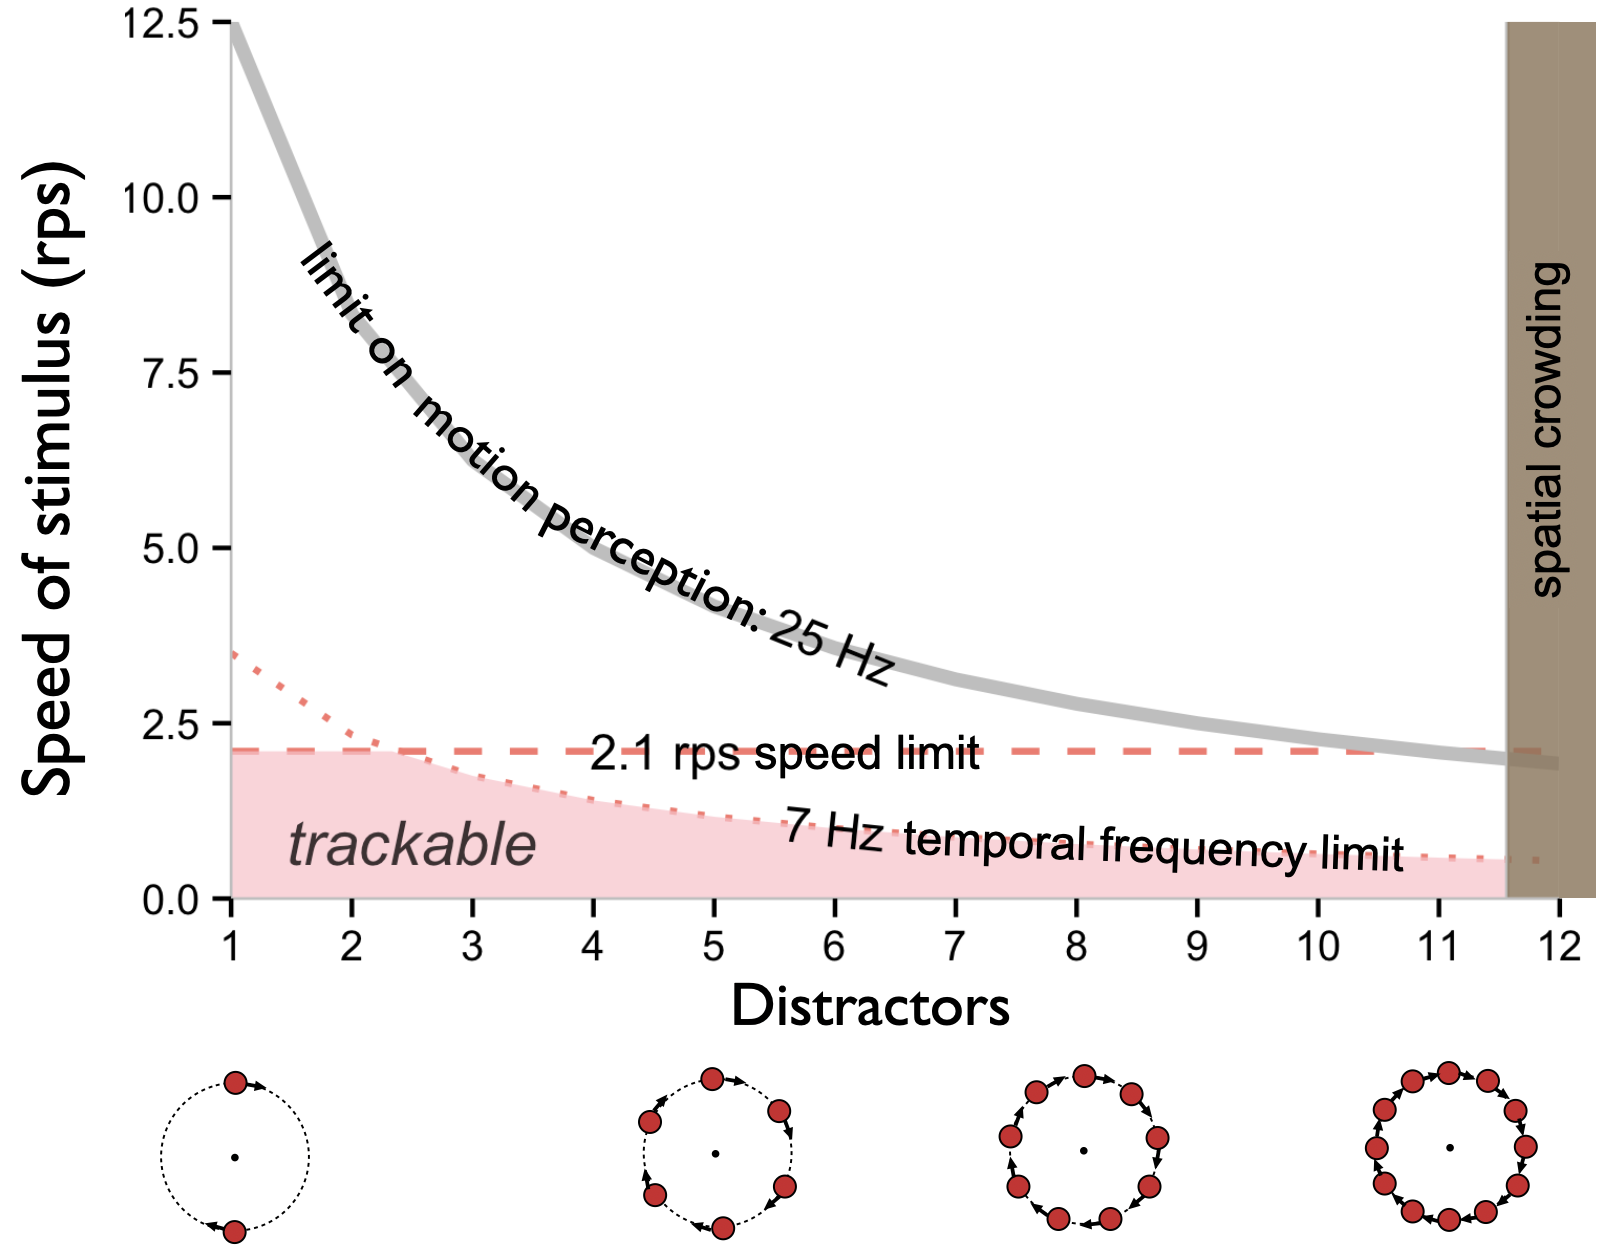
\includegraphics[width=0.9\textwidth,height=\textheight]{imagesForRmd/trackingLimitsMotionLimitSchematic.png}

Because with more targets, these limits overlap a lot, it's still an open question whether speed limits go down just as temporal limits do..

\hypertarget{discarded}{%
\section{Discarded}\label{discarded}}

But what about the role of distractor suppression?

A little bit of motion by

A particular pattern of motion may be key.

The direction of motion of the object changes from time to time, and one must continually update the item's position to know in which of the three locations it ends up.

The limits on tracking are not as simple as a speed limit like we have on the highway. To understand why, we need to start from first principles. In particular we need to consider when attentional tracking is actually needed to do well in a task. If one's target for attention moves only a little bit, tracking probably won't be needed.

When is attentional tracking actually needed to perform well in a tracking task? Motion of the target may not be enough. If targets do not come close to other objects, then one may only need to remember their original location and direction of motion to quickly find them again.

\hypertarget{identity}{%
\chapter{Identity}\label{identity}}

\citet{pylyshynPuzzlingFindingsMultiple2004} ``et in the present studies we show that observers are poor at recalling the identity of successfully tracked objects 􏰞as specified by a unique identifier associated with each target, such as a number or starting location)''

Let's return to the classic shell game. In a shell game, an item is placed beneath one of three identical shells, making that shell the target. The viewer tries to keep track of which shell has the item underneath it.

\begin{figure}
\centering
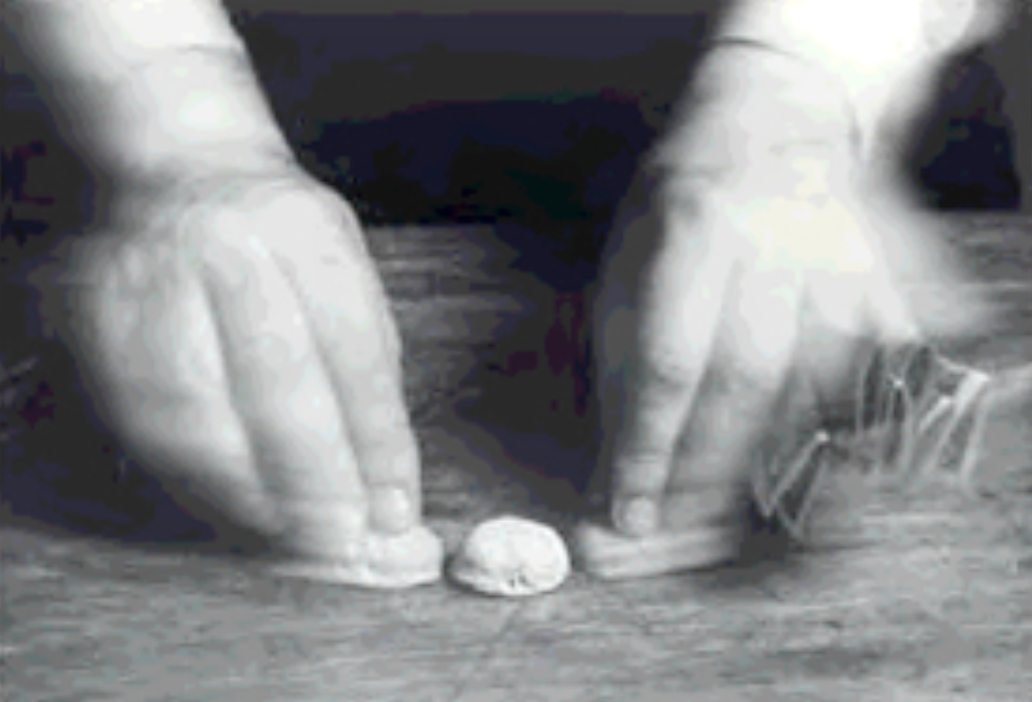
\includegraphics[width=0.5\textwidth,height=\textheight]{imagesForRmd/shellGame.png}
\caption{The location of two identical shells are exchanged in a shell game}
\end{figure}

\hypertarget{tracking-limits-feature-pairing}{%
\section{Tracking limits feature pairing}\label{tracking-limits-feature-pairing}}

movies/MOTmovies/holcombeLinaresVaziriPashkam/pairing.mov

movies/MOTmovies/holcombeLinaresVaziriPashkam/pairing\_3timesfaster.mov

\hypertarget{abilities-individual-differences-dual-task-interference}{%
\chapter{Abilities, individual differences, dual-task interference}\label{abilities-individual-differences-dual-task-interference}}

There are two basic approaches to understanding the abilities that underlie multiple object tracking. One is the classic experimental approach of dissociating the processes involved by manipulating different factors within participants. This has been the dominant approach and has led to our present understanding of the roles of spatial interference, temporal interference, and the duration that one can sustain attention. However, a small but growing literature has used the complementary individual-differences approach. In the individual-differences approach, the pattern of variation in scores on multiple tests is examined to see which abilities tend to go together. Those abilities that co-vary the most are thought to likely share more processes in common than those that don't.

\hypertarget{do-people-vary-much-in-how-many-objects-they-can-track}{%
\section{Do people vary much in how many objects they can track?}\label{do-people-vary-much-in-how-many-objects-they-can-track}}

For some cognitive tasks, individual differences are small, making an individual-differences approach problematic \citep{hedgeReliabilityParadoxWhy2018}. \citet{oksamaMultipleObjectTracking2004} made the effort to test 201 participants on MOT, in an effort to examine variation in how many objects people can track with reasonable accuracy. They found what appeared to be a substantial variation in capacity, with some people able to track six objects, while many could track only two or even just one. However, no analyses were reported regarding the reliability of the MOT test. This left open the possibility that the tracking scores were very noisy, such that the variation in scores found between participants could also have been found if just one participant were tested repeatedly.

Although they did not vary the number of targets participants had to track, \citet{huangMeasuringInterrelationsMultiple2012}, \citet{oksamaMultipleObjectTracking2004}, and \citet{trevinoBridgingCognitiveNeuropsychological} all tested a large number of participants and calculated the correlation in participants' performance between one half of the trials they were tested in and the other. All three found a high correlation of \textgreater{}0.85. Together with their other results and those of \citet{oksamaMultipleObjectTracking2004}, this indicates that people do vary substantially in their multiple object tracking ability.

Variation in MOT performance is typically interpreted by researchers as variation simply in how many objects a person can track.

\hypertarget{what-tasks-are-most-related-to-mot}{%
\section{What tasks are most related to MOT?}\label{what-tasks-are-most-related-to-mot}}

Partly to reveal what other sorts of tasks a high ability to track multiple objects indicates, \citet{huangMeasuringInterrelationsMultiple2012} and \citet{trevinoBridgingCognitiveNeuropsychological} tested large numbers of participants on several tasks. \citet{huangMeasuringInterrelationsMultiple2012} used a set of cognitive and attentional tasks that he termed conjunction search, configuration search, counting, feature access, spatial pattern, response selection, visual short-term memory, change blindness, Raven's test of intelligence, visual marking, attentional capture, consonance-driven orienting, inhibition of return, task switching, mental rotation, and Stroop. While many of these showed high reliability of over .9, the correlations with MOT were moderate, with the highest being counting at 0.4, which required counting the number of white dots in a brief (400 ms) display. Change blindness, feature access, visual working memory, and visual marking were runner ups with correlations of around 0.3.

\citet{trevinoBridgingCognitiveNeuropsychological} reported data from more than 400 participants tested online, and tested a set of cognitive, attentional, and common neuropsychological tasks: arithmetic word problems, the trial-making task, digit span, digit symbol coding, letter cancellation, spatial span, approximate number sense, flanker interference, gradual onset continuous performance, spatial configuration visual search, and visual working memory as well as MOT. MOT had among the highest reliabilities, at 0.92. MOT performance had little correlation with performance on the task designed to measure sustained attention over an extended period (about five minutes, the gradual-onset continual performance task, \citep{fortenbaughSustainedAttentionLife2015}. This supports the tentative conclusion, already suggested in the ``Duration that one can sustain attention'' section of this Element, that the ability to sustain attention without lapses is not an important determinant of tracking performance (as was ).

The tasks with the highest correlations with MOT in the data of \citet{trevinoBridgingCognitiveNeuropsychological} were visual working memory, spatial span, letter cancellation, and digit symbol coding, all at around 0.5. As the authors pointed out, the letter cancellation and digit symbol coding tasks are complex tasks from neuropsychology that are believed to reflect a number of abilities. This makes it hard to interpret their correlation with MOT. Spatial span and visual working memory are quite different from MOT, but similar to each other in that they both involve short-term memory for multiple visual stimuli.

In the \citet{trevinoBridgingCognitiveNeuropsychological} inventory, the task that most resembled the counting task of \citet{huangMeasuringInterrelationsMultiple2012}, which \citet{huangMeasuringInterrelationsMultiple2012} found had a high correlation with MOT, was the approximate number sense task, with a moderate correlation of 0.3. It differed from the counting task of \citet{huangMeasuringInterrelationsMultiple2012} by not testing the subitizing (less than 5 items) range, which might help explain any discrepancy. In a more limited study, \citet{eayrsEstablishingIndividualDifferences2018} found, using hierarchical regression, that subitizing made a contribution to predicting MOT performance that was somewhat separate to that of an estimation task using larger set sizes.

Overall, there is a reasonable level of agreement across these individual-differences studies, as well as others not described here, such as \citet{trickSpatialVisuospatialWorking2012}. They agree that visual working memory has a robust correlation with MOT performance, which is particularly interesting because superficially, MOT imposes little to no memory demand. Most researchers conceive of tracking as involving allocating multifocal attention to multiple targets simultaneously, with a process autonomous to memory causing the foci of attention to move along with the moving targets.

``Working memory is a well-established predictor of individual differences in a range of attention tasks, including for example the Stroop task, spatial cuing and task switching (e.g.~Kane \& Engle, 2001; Kane, Bleckley, Conway \& Engle, 2001; Redick \& Engle, 2006).''

With the growth of online testing, we can expect this approach to

\hypertarget{dual-task}{%
\section{Dual-task}\label{dual-task}}

The dual-task literature is very large. Can't review it all here

There seems to be an especially close link between MOT and subitizing
\citet{trickAgeDifferencesEnumerating2003} observed that even very slow motion reduced
enumeration speed for stimuli containing 6--9 items, while
the enumeration of 1--4 items was not affected when items
were in motion. Similarly, \citet{alstonSubitizationAttentionalEngagement2004}
presented static and moving items, finding that faster and
more accurate enumeration occurred in the subitizing range
given the presence of moving items.

Subitizing no bilateral advantage on accuracy, but that could be due to very high accuracy - when looking at response time, an advantage is found, although not clear it's as large as that for MOT \citet{railoBilateralTwoitemAdvantage2014}

``The results indicated that the number of items participants could subitize decreased by one for each item they tracked.'' \citet{chesneyEvidenceSharedMechanism2011}

``concurrent performance of a MOT task and a VWM task still instilled substantial and load-dependent dual-task costs.'' \citet{fougnieDistinctCapacityLimits2006}

\citet{allenMultipletargetTrackingRole2006}

psilocybin seems to impair MOT but not visual working memory \citep{carterUsingPsilocybinInvestigate2005}

object tracking in people with Williams Syndrome remains at the level of 4‐year‐olds, whereas the ability to remember multiple locations of static objects develops further. \citet{ohearnDevelopmentalProfilesMultiple2010}

\citet{howardVisualSpatialAttention2020} ``for a purely spatial task, perceptual attention (TRACKING?) and working memory appear to recruit separate core capacity-limited processes.''

\citet{souzaContributionsVisualCentral2017} argued that VWM and MOT use different attentional resources." ``Distracting visual attention, but not central attention, impaired MOT performance''

\hypertarget{real-world}{%
\chapter{Real world}\label{real-world}}

\citet{harrisExaminingRolesWorking2020} low N comparing sports players

\citet{mangineVisualTrackingSpeed2014} Twelve professional basketball players were tested before the 2012--13 season. Visual tracking speed was obtained from 1 core session (20 trials) of the multiple object tracking test, whereas RT was measured by fixed- and variable-region choice reaction tests, using a light-based testing device. Performance in VTS and RT was compared with basketball-specific measures of performance (assists {[}AST{]}; turnovers {[}TO{]}; assist-to-turnover ratio {[}AST/TO{]}; steals {[}STL{]}) during the regular basketball season. All performance measures were reported per 100 minutes played. Performance differences between backcourt (guards; n = 5) and frontcourt (forward/centers; n = 7\ldots{}

Study of only 12 pro basketball players finding correlations with basketball metrics \citet{mangineVisualTrackingSpeed2014}

\hypertarget{misconceptions-and-questions}{%
\chapter{Misconceptions and questions}\label{misconceptions-and-questions}}

Top misconceptions about MOT
* its capacity limit is around 4 items.(this has been used to argue that it has a similar capacity limit to visual working memory (Cowan, 2001).)
* ``While the most intuitive model of multiple object tracking would involve storing the locations of targets in spatial memory, then moving attention in turn as quickly as possible to each target to update its location, this class of model is unable to account for MOT performance (Pylyshyn \& Storm, 1988; Vul et al., 2009)''

Reading your paper also gave me an idea to have a Common Misconceptions section for the Cambridge Element.~ One might be that the capacity limit on VWM and MOT coincide (what you refer to as ``The most striking link between the two tasks is that they seem to have a similar capacity limit of around four items (Cowan, 2001)''. I totally agree that it is striking and so it is natural to think it means something, but while I don't know much about VWM, the capacity limit for MOT is determined by the speeds, spatial proximities,and temporal frequencies~used,~so as you know the limit can be anything between zero and more than ten.~ It is true that the speeds most often used yield a capacity limit of around four, but I haven't seen any argument for why the commonly used speeds/spatial proximities/temporal frequency combination is more special than the other possibilities. I guess one could argue that researchers set those parameters to resemble an intuition for what real-world tasks are like, but even if they got that right, I'm not sure the same is true for VWM setups, or what that would imply for underlying ability structures. It seems to me one would have to do some kind of ideal observer (really, ideal thinker) model with the same assumptions that can model both common VWM and common MOT tasks, and show that the same level of ability in fundamental processes underlying each would yield the same capacity limit of four in both cases.

Thus, while many potential athlete users may imagine that a test of attention tests how long they can pay attention, this is not likely to be the reason for differences among people on MOT performance.

\hypertarget{topics-not-covered-by-this-review}{%
\section{Topics not covered by this review}\label{topics-not-covered-by-this-review}}

Retinotopic or spatiotopic and configural \citet{yantisMultielementVisualTracking1992}, \citet{billHierarchicalStructureEmployed2020}, \citet{howeCoordinateSystemsUsed2010}

expansion and contraction hurts position judgments \citet{howeVisuallyTrackingLocalizing2013}

Role of surface features \citet{papenmeierTrackingLocationFeatures2014}

\bibliography{CambridgeElement.bib,packages.bib}

\end{document}
